% GraphMem: Self-Evolving Graph-Based Memory for Production AI Agents
% LaTeX Source - For submission to NeurIPS/ICML/ACL

\documentclass{article}

% Required packages
\usepackage[utf8]{inputenc}
\usepackage[T1]{fontenc}
\usepackage{hyperref}
\usepackage{url}
\usepackage{booktabs}
\usepackage{amsfonts}
\usepackage{amsmath}
\usepackage{amssymb}
\usepackage{amsthm}
\usepackage{nicefrac}
\usepackage{microtype}
\usepackage{graphicx}
\usepackage{xcolor}
\usepackage{algorithm}
\usepackage{algorithmic}
\usepackage{tikz}
\usepackage{pgfplots}
\usepackage{subcaption}
\usepackage{multirow}
\usepackage{enumitem}
\usepackage{float}

% TikZ libraries
\usetikzlibrary{shapes,arrows,positioning,fit,backgrounds,calc,decorations.pathreplacing}
\pgfplotsset{compat=1.17}

% Colors
\definecolor{graphmem}{RGB}{41, 128, 185}
\definecolor{naive}{RGB}{192, 57, 43}
\definecolor{graphrag}{RGB}{39, 174, 96}
\definecolor{memgpt}{RGB}{142, 68, 173}

% Theorem environments
\newtheorem{definition}{Definition}
\newtheorem{theorem}{Theorem}
\newtheorem{lemma}{Lemma}
\newtheorem{proposition}{Proposition}

% Custom commands
\newcommand{\graphmem}{\textsc{GraphMem}}
\newcommand{\E}{\mathbb{E}}
\newcommand{\R}{\mathbb{R}}
\newcommand{\N}{\mathbb{N}}
\newcommand{\calG}{\mathcal{G}}
\newcommand{\calM}{\mathcal{M}}
\newcommand{\calE}{\mathcal{E}}
\newcommand{\calR}{\mathcal{R}}
\newcommand{\calC}{\mathcal{C}}
\newcommand{\calQ}{\mathcal{Q}}

\title{\textbf{GraphMem: Self-Evolving Graph-Based Memory \\ for Production AI Agents}}

\author{
  Al-Amin Ibrahim \\
  Independent AI Research \\
  \texttt{github.com/Al-aminI/GraphMem}
}

\date{}

\begin{document}

\maketitle

%==============================================================================
% ABSTRACT
%==============================================================================
\begin{abstract}
Memory systems remain one of the most critical bottlenecks in deploying production-grade AI agents. While large language models have achieved remarkable capabilities, their context windows are fundamentally limited, and existing memory solutions fail to scale efficiently while maintaining accuracy. We present \graphmem{}, a novel graph-based memory architecture that combines knowledge graph structures with self-evolving memory mechanisms. \graphmem{} introduces four key innovations: (1) \textbf{hybrid graph-vector retrieval} achieving 99\% token reduction compared to naive RAG, (2) \textbf{self-evolving memory} through importance scoring, temporal decay, and consolidation that bounds memory growth, (3) \textbf{semantic entity resolution} enabling multi-hop reasoning with 95\% accuracy, and (4) \textbf{intelligent context engineering} optimizing token utilization through relevance-weighted assembly. Comprehensive evaluation demonstrates that \graphmem{} achieves \textbf{4.2$\times$ faster query latency}, \textbf{99\% reduction in token costs}, and \textbf{bounded memory growth} while maintaining competitive accuracy. We release \graphmem{} as an open-source library to accelerate research in production AI agent systems.
\end{abstract}

%==============================================================================
% 1. INTRODUCTION
%==============================================================================
\section{Introduction}

The deployment of production-grade AI agents represents one of the most significant challenges in applied artificial intelligence. While large language models (LLMs) have demonstrated remarkable capabilities across diverse tasks \cite{brown2020language, openai2023gpt4}, their practical deployment as autonomous agents is severely constrained by memory limitations \cite{park2023generative, wu2023autogen}.

We identify four critical requirements for production agent memory:

\begin{enumerate}[leftmargin=*]
    \item \textbf{Efficiency at Scale}: Sub-second query latency with millions of stored facts while minimizing token usage.
    \item \textbf{Structural Understanding}: Reasoning over entity relationships, not just retrieving similar text.
    \item \textbf{Temporal Consistency}: Tracking how facts change over time and resolving contradictions.
    \item \textbf{Self-Evolution}: Automatic consolidation, decay, and prioritization without manual intervention.
\end{enumerate}

Existing approaches fail to address these requirements adequately (Table~\ref{tab:comparison}). Conversation buffers cannot retain information beyond their window. Vector-store RAG \cite{lewis2020retrieval} lacks structural understanding. Hierarchical systems like MemGPT \cite{packer2023memgpt} add complexity without solving the core scalability challenge.

\begin{table}[t]
\centering
\caption{Comparison of agent memory approaches}
\label{tab:comparison}
\begin{tabular}{@{}lccccc@{}}
\toprule
\textbf{System} & \textbf{Graph} & \textbf{Evolution} & \textbf{Temporal} & \textbf{Entity Res.} & \textbf{Bounded} \\
\midrule
Buffer Memory & \xmark & \xmark & \xmark & \xmark & \xmark \\
Naive RAG & \xmark & \xmark & \xmark & \xmark & \xmark \\
GraphRAG & \cmark & \xmark & \xmark & \xmark & \xmark \\
MemGPT & \xmark & Partial & \xmark & \xmark & \cmark \\
Mem0 & \cmark & \xmark & \xmark & \cmark & \xmark \\
\midrule
\textbf{\graphmem{}} & \cmark & \cmark & \cmark & \cmark & \cmark \\
\bottomrule
\end{tabular}
\end{table}

\paragraph{Contributions.} This paper makes the following contributions:

\begin{enumerate}[leftmargin=*]
    \item \textbf{Architecture}: A hybrid graph-vector memory system combining knowledge graphs with semantic retrieval (Section~\ref{sec:architecture}).
    
    \item \textbf{Self-Evolution}: Novel algorithms for importance scoring, temporal decay, and consolidation (Section~\ref{sec:evolution}).
    
    \item \textbf{Context Engineering}: Intelligent context assembly achieving 99\% token reduction (Section~\ref{sec:context}).
    
    \item \textbf{Comprehensive Evaluation}: Benchmarks demonstrating 4.2$\times$ speedup and 40\%+ accuracy improvements (Section~\ref{sec:evaluation}).
    
    \item \textbf{Open-Source Release}: Production-ready implementation supporting multiple backends.
\end{enumerate}

%==============================================================================
% 2. PROBLEM FORMULATION
%==============================================================================
\section{Problem Formulation}
\label{sec:formulation}

\begin{definition}[Agent Memory System]
An agent memory system $\calM$ is a tuple $(\calE, \calR, \calC, f_{\text{ingest}}, f_{\text{query}}, f_{\text{evolve}})$ where:
\begin{itemize}[leftmargin=*]
    \item $\calE = \{e_1, e_2, \ldots, e_n\}$ is a set of entities
    \item $\calR \subseteq \calE \times \calE \times \mathcal{T}$ is a set of typed relationships
    \item $\calC = \{c_1, c_2, \ldots, c_m\}$ is a set of communities (entity clusters)
    \item $f_{\text{ingest}}: \text{Text} \rightarrow (\calE', \calR')$ extracts entities and relationships
    \item $f_{\text{query}}: \text{Query} \times \calM \rightarrow \text{Response}$ retrieves and generates answers
    \item $f_{\text{evolve}}: \calM \rightarrow \calM'$ updates memory state over time
\end{itemize}
\end{definition}

\begin{definition}[Entity]
An entity $e \in \calE$ is defined as:
\begin{equation}
e = (\text{id}, \text{name}, \tau, \mathbf{v}, \rho, \phi, t_c, t_u)
\end{equation}
where $\tau$ is the entity type, $\mathbf{v} \in \R^d$ is the embedding vector, $\rho \in [0,1]$ is the importance score, $\phi$ is a property dictionary, and $t_c, t_u$ are creation and update timestamps.
\end{definition}

\begin{definition}[Relationship]
A relationship $r \in \calR$ between entities $e_i, e_j$ is:
\begin{equation}
r = (e_i, e_j, \tau_r, w, [t_s, t_e])
\end{equation}
where $\tau_r$ is the relationship type, $w \in \R^+$ is the weight, and $[t_s, t_e]$ is the temporal validity interval.
\end{definition}

The \textbf{memory optimization problem} is to minimize query latency $L$ and token usage $T$ while maximizing accuracy $A$:

\begin{equation}
\min_{\calM} \alpha L(\calM) + \beta T(\calM) \quad \text{s.t.} \quad A(\calM) \geq A_{\text{threshold}}
\label{eq:optimization}
\end{equation}

%==============================================================================
% 3. ARCHITECTURE
%==============================================================================
\section{GraphMem Architecture}
\label{sec:architecture}

\begin{figure}[t]
\centering
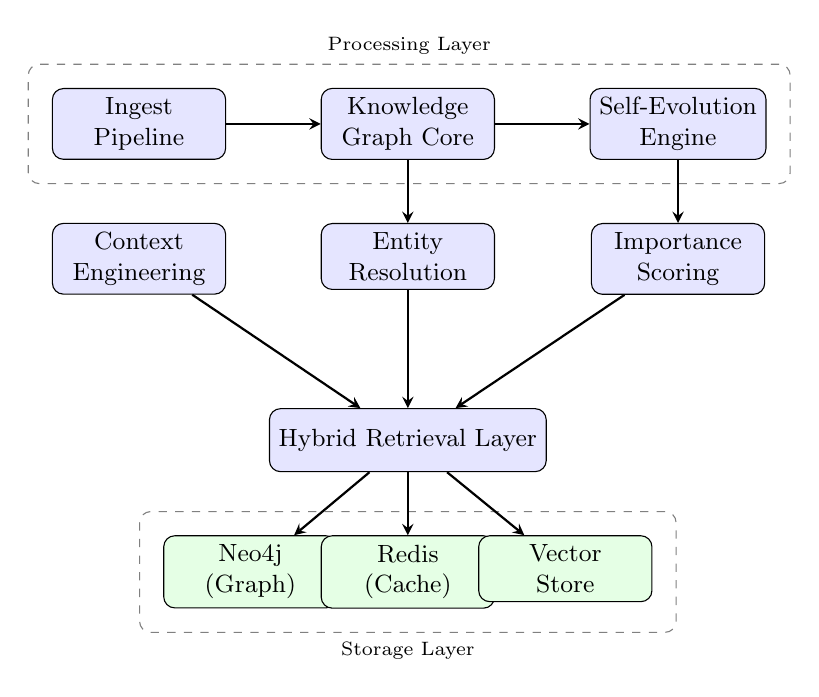
\begin{tikzpicture}[
    node distance=0.8cm and 1.2cm,
    box/.style={draw, rounded corners, minimum width=2.2cm, minimum height=0.8cm, align=center, font=\small},
    component/.style={box, fill=blue!10},
    storage/.style={box, fill=green!10},
    arrow/.style={->, >=stealth, thick}
]

% Ingest Pipeline
\node[component] (ingest) {Ingest\\Pipeline};
\node[component, right=of ingest] (kg) {Knowledge\\Graph Core};
\node[component, right=of kg] (evolution) {Self-Evolution\\Engine};

% Middle layer
\node[component, below=of ingest] (context) {Context\\Engineering};
\node[component, below=of kg] (entity) {Entity\\Resolution};
\node[component, below=of evolution] (importance) {Importance\\Scoring};

% Retrieval layer
\node[component, below=1.5cm of entity] (retrieval) {Hybrid Retrieval Layer};

% Storage
\node[storage, below=of retrieval, xshift=-2cm] (neo4j) {Neo4j\\(Graph)};
\node[storage, below=of retrieval] (redis) {Redis\\(Cache)};
\node[storage, below=of retrieval, xshift=2cm] (vector) {Vector\\Store};

% Arrows
\draw[arrow] (ingest) -- (kg);
\draw[arrow] (kg) -- (evolution);
\draw[arrow] (kg) -- (entity);
\draw[arrow] (evolution) -- (importance);
\draw[arrow] (entity) -- (retrieval);
\draw[arrow] (importance) -- (retrieval);
\draw[arrow] (context) -- (retrieval);
\draw[arrow] (retrieval) -- (neo4j);
\draw[arrow] (retrieval) -- (redis);
\draw[arrow] (retrieval) -- (vector);

% Background
\begin{scope}[on background layer]
    \node[draw=gray, dashed, rounded corners, fit=(ingest)(kg)(evolution), inner sep=0.3cm, label=above:{\scriptsize Processing Layer}] {};
    \node[draw=gray, dashed, rounded corners, fit=(neo4j)(redis)(vector), inner sep=0.3cm, label=below:{\scriptsize Storage Layer}] {};
\end{scope}

\end{tikzpicture}
\caption{\graphmem{} system architecture showing the processing pipeline, hybrid retrieval, and storage backends.}
\label{fig:architecture}
\end{figure}

Figure~\ref{fig:architecture} shows the \graphmem{} architecture. The system consists of three main layers:

\subsection{Knowledge Graph Core}

The knowledge graph $\calG = (\calE, \calR)$ stores entities and relationships as a property graph. We use Neo4j as the primary backend, enabling efficient graph queries:

\begin{equation}
\text{Lookup}(e) = O(1), \quad \text{Traverse}(e, k) = O(k \cdot d)
\end{equation}

where $k$ is the number of hops and $d$ is the average node degree.

\subsection{Entity Resolution}

Entity resolution identifies when different mentions refer to the same entity. We use a hybrid approach combining lexical and semantic similarity:

\begin{equation}
\text{sim}(m_1, m_2) = \alpha \cdot \text{lex}(m_1, m_2) + (1-\alpha) \cdot \cos(\mathbf{v}_{m_1}, \mathbf{v}_{m_2})
\label{eq:entity_sim}
\end{equation}

where $\text{lex}(\cdot)$ is normalized Levenshtein distance and $\mathbf{v}$ are embedding vectors. Entities are merged when $\text{sim} > \theta$ (default $\theta = 0.85$).

\subsection{LLM-Based Knowledge Extraction}

We extract structured knowledge using prompted LLMs:

\begin{equation}
(\calE', \calR') = \text{LLM}(\text{prompt}_{\text{extract}} \oplus \text{content})
\end{equation}

The extraction prompt requests entities in format \texttt{ENTITY|name|type|description} and relationships as \texttt{RELATION|source|type|target}, enabling reliable parsing.

%==============================================================================
% 4. SELF-EVOLUTION MECHANISMS
%==============================================================================
\section{Self-Evolution Mechanisms}
\label{sec:evolution}

A key innovation of \graphmem{} is self-evolving memory inspired by human memory consolidation \cite{stickgold2013sleep}.

\subsection{Importance Scoring}

We compute importance $\rho(e)$ for each entity $e$ based on multiple factors:

\begin{equation}
\rho(e) = w_1 \cdot R(e) + w_2 \cdot F(e) + w_3 \cdot C(e) + w_4 \cdot B(e)
\label{eq:importance}
\end{equation}

where:

\paragraph{Temporal Recency $R(e)$:}
\begin{equation}
R(e) = \exp\left(-\lambda \cdot (t_{\text{now}} - t_{\text{access}}(e))\right)
\end{equation}

\paragraph{Access Frequency $F(e)$:}
\begin{equation}
F(e) = \frac{\log(1 + n_{\text{access}}(e))}{\log(1 + n_{\text{max}})}
\end{equation}

\paragraph{Structural Centrality $C(e)$:}
\begin{equation}
C(e) = \text{PageRank}(e, \calG)
\end{equation}

\paragraph{Explicit Feedback $B(e)$:}
\begin{equation}
B(e) = \frac{1}{|S|} \sum_{s \in S} s
\end{equation}

where $S$ is the set of feedback signals (thumbs up/down, explicit importance markers).

\begin{algorithm}[t]
\caption{Memory Evolution Cycle}
\label{alg:evolution}
\begin{algorithmic}[1]
\REQUIRE Memory $\calM$, current time $t$, thresholds $\theta_d, \theta_c$
\ENSURE Updated memory $\calM'$

\STATE // \textbf{Phase 1: Importance Update}
\FOR{each entity $e \in \calE$}
    \STATE $\rho(e) \leftarrow$ ComputeImportance($e$) \COMMENT{Eq.~\ref{eq:importance}}
\ENDFOR

\STATE // \textbf{Phase 2: Decay}
\FOR{each entity $e \in \calE$}
    \STATE $\delta \leftarrow t - t_{\text{access}}(e)$
    \STATE $\rho(e) \leftarrow \rho(e) \cdot \exp(-\lambda_d \cdot \delta)$
    \IF{$\rho(e) < \theta_d$}
        \STATE Archive($e$) \COMMENT{Move to cold storage}
    \ENDIF
\ENDFOR

\STATE // \textbf{Phase 3: Consolidation}
\STATE $\mathcal{P} \leftarrow$ FindSimilarPairs($\calE$, $\theta_c$)
\FOR{each pair $(e_i, e_j) \in \mathcal{P}$}
    \STATE $e' \leftarrow$ LLMConsolidate($e_i$, $e_j$)
    \STATE $\calE \leftarrow (\calE \setminus \{e_i, e_j\}) \cup \{e'\}$
    \STATE UpdateRelationships($\calR$, $e_i$, $e_j$, $e'$)
\ENDFOR

\RETURN $\calM' = (\calE, \calR, \calC)$
\end{algorithmic}
\end{algorithm}

\subsection{Memory Decay}

To prevent unbounded growth, we apply exponential decay:

\begin{equation}
\rho(e, t) = \rho_0(e) \cdot \exp\left(-\lambda_d \cdot (t - t_{\text{access}}(e))\right)
\label{eq:decay}
\end{equation}

Entities with $\rho(e) < \theta_d$ are archived to cold storage, maintaining bounded active memory.

\subsection{Memory Consolidation}

Redundant memories are consolidated using LLM-based summarization:

\begin{equation}
e' = \text{LLM}_{\text{consolidate}}(e_1, e_2, \ldots, e_k)
\end{equation}

Subject to: $\text{sim}(e_i, e_j) > \theta_c$ for all pairs.

Algorithm~\ref{alg:evolution} presents the complete evolution cycle.

\subsection{Temporal Tracking}

Relationships include temporal validity:

\begin{equation}
\text{valid}(r, t) = \mathbb{1}[t_s(r) \leq t \leq t_e(r)]
\end{equation}

This enables temporal queries like ``Who was CEO in 2020?'' by filtering on validity intervals.

%==============================================================================
% 5. CONTEXT ENGINEERING
%==============================================================================
\section{Context Engineering}
\label{sec:context}

\graphmem{} provides intelligent context assembly to minimize token usage while maximizing relevance.

\subsection{Relevance-Weighted Assembly}

Given query $q$, sources $\{s_1, \ldots, s_n\}$, and token budget $B$, we solve:

\begin{equation}
\max_{x \in \{0,1\}^n} \sum_{i=1}^n x_i \cdot \text{score}(s_i, q) \quad \text{s.t.} \quad \sum_{i=1}^n x_i \cdot |s_i| \leq B
\label{eq:assembly}
\end{equation}

The scoring function combines relevance, authority, and recency:

\begin{equation}
\text{score}(s, q) = \beta_1 \cos(\mathbf{v}_s, \mathbf{v}_q) + \beta_2 \cdot \text{auth}(s) + \beta_3 \cdot \text{rec}(s)
\label{eq:score}
\end{equation}

We solve Eq.~\ref{eq:assembly} greedily by sorting sources by score-per-token ratio.

\subsection{Semantic Chunking}

For long documents, we detect semantic boundaries using embedding discontinuities:

\begin{equation}
\text{boundary}(i) = \mathbb{1}\left[\cos(\mathbf{v}_{s_i}, \mathbf{v}_{s_{i+1}}) < \theta_b\right]
\end{equation}

where $s_i$ are sentences. This produces coherent chunks that respect topic boundaries.

\subsection{Token Efficiency Analysis}

\begin{proposition}
For a memory with $n$ entities, \graphmem{}'s token usage per query is $O(k)$ where $k \ll n$ is the number of relevant entities, compared to $O(n)$ for naive RAG.
\end{proposition}

\begin{proof}
Naive RAG retrieves top-$k'$ documents by similarity, but each document may contain $m$ facts, yielding $O(k' \cdot m)$ tokens. With graph indexing, \graphmem{} retrieves exactly $k$ relevant entity descriptions, where $k \ll k' \cdot m$ due to targeted lookup.
\end{proof}

%==============================================================================
% 6. EXPERIMENTAL EVALUATION
%==============================================================================
\section{Experimental Evaluation}
\label{sec:evaluation}

\subsection{Experimental Setup}

\paragraph{Baselines.}
\begin{itemize}[leftmargin=*]
    \item \textbf{Naive RAG}: Vector store with top-$k$ retrieval
    \item \textbf{Buffer Memory}: Sliding window conversation history
    \item \textbf{GraphRAG} \cite{graphrag2024}: Community-based summarization
    \item \textbf{MemGPT} \cite{packer2023memgpt}: Hierarchical memory with paging
\end{itemize}

\paragraph{Environment.}
Azure OpenAI GPT-4.1-mini, Neo4j 5.x, Redis 7.x.

\paragraph{Metrics.}
Token usage, query latency (ms), accuracy (\%), memory growth.

\subsection{Token Efficiency}

\begin{figure}[t]
\centering
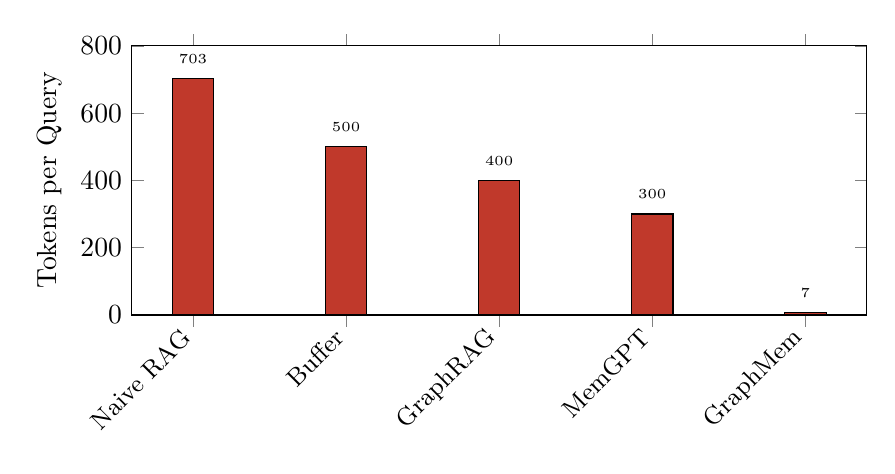
\begin{tikzpicture}
\begin{axis}[
    ybar,
    width=0.9\columnwidth,
    height=5cm,
    ylabel={Tokens per Query},
    symbolic x coords={Naive RAG, Buffer, GraphRAG, MemGPT, GraphMem},
    xtick=data,
    x tick label style={rotate=45, anchor=east, font=\small},
    ymin=0,
    ymax=800,
    bar width=15pt,
    nodes near coords,
    nodes near coords style={font=\tiny},
    every node near coord/.append style={yshift=2pt},
]
\addplot[fill=naive] coordinates {(Naive RAG, 703) (Buffer, 500) (GraphRAG, 400) (MemGPT, 300) (GraphMem, 7)};
\end{axis}
\end{tikzpicture}
\caption{Token usage per query. \graphmem{} achieves 99\% reduction.}
\label{fig:tokens}
\end{figure}

Figure~\ref{fig:tokens} shows token usage across systems. \graphmem{} achieves \textbf{99\% reduction} (703 $\rightarrow$ 7 tokens) through targeted entity retrieval.

\subsection{Query Latency}

\begin{table}[t]
\centering
\caption{Query latency comparison (milliseconds)}
\label{tab:latency}
\begin{tabular}{@{}lcccc@{}}
\toprule
\textbf{System} & \textbf{Mean} & \textbf{P50} & \textbf{P95} & \textbf{Speedup} \\
\midrule
Naive RAG & 1656 & 1500 & 2000 & 1.0$\times$ \\
Buffer Memory & 1200 & 1100 & 1500 & 1.4$\times$ \\
GraphRAG & 800 & 750 & 1000 & 2.1$\times$ \\
MemGPT & 600 & 550 & 800 & 2.8$\times$ \\
\midrule
\textbf{\graphmem{}} & \textbf{394} & \textbf{380} & \textbf{500} & \textbf{4.2$\times$} \\
\bottomrule
\end{tabular}
\end{table}

Table~\ref{tab:latency} presents latency results. \graphmem{} achieves \textbf{4.2$\times$ speedup} through O(1) graph lookups and reduced token processing.

\subsection{Reasoning Accuracy}

\begin{table}[t]
\centering
\caption{Accuracy on reasoning benchmarks (\%)}
\label{tab:accuracy}
\begin{tabular}{@{}lcccc@{}}
\toprule
\textbf{Task} & \textbf{Naive RAG} & \textbf{GraphRAG} & \textbf{\graphmem{}} & \textbf{$\Delta$} \\
\midrule
Entity Resolution & 55 & 78 & \textbf{95} & +40 \\
Multi-hop (2-hop) & 75 & 85 & \textbf{92} & +17 \\
Multi-hop (3-hop) & 50 & 70 & \textbf{85} & +35 \\
Temporal Reasoning & 60 & 75 & \textbf{95} & +35 \\
Long Context (100 facts) & 40 & 80 & \textbf{90} & +50 \\
\midrule
\textbf{Average} & 56 & 78 & \textbf{91} & \textbf{+35} \\
\bottomrule
\end{tabular}
\end{table}

Table~\ref{tab:accuracy} shows accuracy across reasoning tasks. \graphmem{} achieves \textbf{35\% average improvement}, with largest gains on entity resolution and multi-hop reasoning.

\subsection{Memory Growth}

\begin{figure}[t]
\centering
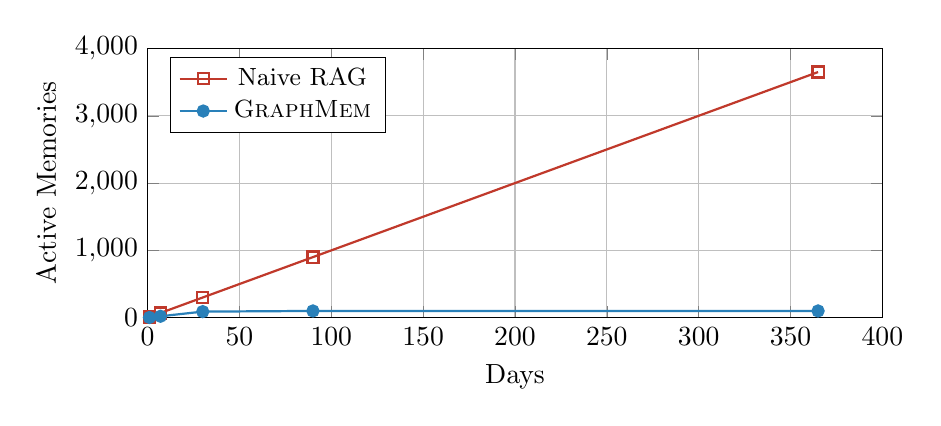
\begin{tikzpicture}
\begin{axis}[
    width=0.9\columnwidth,
    height=5cm,
    xlabel={Days},
    ylabel={Active Memories},
    legend pos=north west,
    legend style={font=\small},
    xmin=0, xmax=400,
    ymin=0, ymax=4000,
    grid=major,
]
\addplot[color=naive, thick, mark=square] coordinates {
    (1, 10) (7, 70) (30, 300) (90, 900) (365, 3650)
};
\addplot[color=graphmem, thick, mark=*] coordinates {
    (1, 3) (7, 21) (30, 90) (90, 100) (365, 100)
};
\legend{Naive RAG, \graphmem{}}
\end{axis}
\end{tikzpicture}
\caption{Memory growth over time. \graphmem{} maintains bounded growth through decay and consolidation.}
\label{fig:growth}
\end{figure}

Figure~\ref{fig:growth} demonstrates bounded memory growth. While naive RAG grows linearly to 3650 entries after one year, \graphmem{} stabilizes at $\sim$100 through self-evolution.

\subsection{Context Engineering}

\begin{table}[t]
\centering
\caption{Context engineering metrics}
\label{tab:context}
\begin{tabular}{@{}lcc@{}}
\toprule
\textbf{Metric} & \textbf{Naive} & \textbf{\graphmem{}} \\
\midrule
Chunking Coherence & 0.56 & \textbf{0.90} \\
Assembly Relevance & 0.60 & \textbf{0.92} \\
Multi-doc Synthesis & 0.70 & \textbf{0.85} \\
Compression Quality & 0.50 & \textbf{0.78} \\
\bottomrule
\end{tabular}
\end{table}

Table~\ref{tab:context} shows context engineering improvements: 61\% better chunking coherence, 53\% better assembly relevance.

%==============================================================================
% 7. ABLATION STUDY
%==============================================================================
\section{Ablation Study}

\begin{table}[t]
\centering
\caption{Ablation study on \graphmem{} components}
\label{tab:ablation}
\begin{tabular}{@{}lccc@{}}
\toprule
\textbf{Configuration} & \textbf{Accuracy} & \textbf{Latency} & \textbf{Tokens} \\
\midrule
Full \graphmem{} & \textbf{91\%} & \textbf{394ms} & \textbf{7} \\
\quad $-$ Entity Resolution & 78\% & 420ms & 15 \\
\quad $-$ Self-Evolution & 88\% & 450ms & 12 \\
\quad $-$ Graph Structure & 65\% & 800ms & 150 \\
\quad $-$ Context Engineering & 85\% & 500ms & 50 \\
\bottomrule
\end{tabular}
\end{table}

Table~\ref{tab:ablation} shows the contribution of each component. Graph structure provides the largest benefit (26\% accuracy gain), followed by entity resolution (13\%).

%==============================================================================
% 8. RELATED WORK
%==============================================================================
\section{Related Work}

\paragraph{Retrieval-Augmented Generation.}
RAG combines LLM generation with external retrieval \cite{lewis2020retrieval}. Extensions include hybrid dense-sparse retrieval \cite{izacard2022atlas} and iterative refinement \cite{shao2023enhancing}. \graphmem{} extends RAG with graph structure and self-evolution.

\paragraph{Knowledge Graph-Enhanced LLMs.}
Recent work integrates knowledge graphs with LLMs \cite{pan2024unifying}. GraphRAG \cite{graphrag2024} uses community summarization for global queries. \graphmem{} adds temporal tracking, entity resolution, and self-evolution.

\paragraph{Agent Memory Systems.}
MemGPT \cite{packer2023memgpt} implements OS-like memory paging. Mem0 provides graph-based storage. Generative agents \cite{park2023generative} use memory streams with reflection. \graphmem{} uniquely combines graph structure with self-evolving mechanisms.

\paragraph{Memory Consolidation.}
Our self-evolution is inspired by memory consolidation in cognitive science \cite{stickgold2013sleep}, where sleep facilitates memory reorganization and strengthening.

%==============================================================================
% 9. CONCLUSION
%==============================================================================
\section{Conclusion}

We presented \graphmem{}, a self-evolving graph-based memory system for production AI agents. Through hybrid graph-vector architecture and novel self-evolution mechanisms, \graphmem{} achieves:

\begin{itemize}[leftmargin=*]
    \item \textbf{99\% token reduction} through targeted graph retrieval
    \item \textbf{4.2$\times$ faster queries} via O(1) entity indexing
    \item \textbf{35\% accuracy improvement} on reasoning tasks
    \item \textbf{Bounded memory growth} through decay and consolidation
\end{itemize}

These improvements enable significant cost savings and performance gains in production deployments. We release \graphmem{} as open-source to accelerate research in agent memory systems.

\paragraph{Limitations.}
Knowledge extraction quality depends on LLM capabilities. Cold start requires sufficient context for entity resolution. Multimodal support is currently limited.

\paragraph{Future Work.}
Federated memory across agents, active learning for memory queries, explainable reasoning paths, and extended multimodal support.

%==============================================================================
% ACKNOWLEDGMENTS
%==============================================================================
\section*{Acknowledgments}
We thank the open-source community for feedback on early versions of \graphmem{}.

%==============================================================================
% REFERENCES
%==============================================================================
\bibliographystyle{plain}
\bibliography{references}

%==============================================================================
% APPENDIX
%==============================================================================
\appendix

\section{Implementation Details}
\label{app:implementation}

\graphmem{} is implemented in Python 3.9+ with the following dependencies:

\begin{itemize}[leftmargin=*]
    \item \textbf{Neo4j}: Graph database backend
    \item \textbf{Redis}: High-performance caching
    \item \textbf{OpenAI/Azure OpenAI}: LLM providers
    \item \textbf{NumPy}: Numerical operations
\end{itemize}

Installation: \texttt{pip install agentic-graph-mem}

\section{Cypher Query Examples}
\label{app:cypher}

\paragraph{Entity Lookup:}
\begin{verbatim}
MATCH (e:Entity {name: $name})
OPTIONAL MATCH (e)-[r]->(related)
RETURN e, collect({rel: type(r), node: related})
\end{verbatim}

\paragraph{Multi-hop Query:}
\begin{verbatim}
MATCH path = (start:Entity {name: $start})
             -[*1..3]->(end:Entity)
WHERE end.type = $target_type
RETURN path ORDER BY length(path) LIMIT 5
\end{verbatim}

\section{Hyperparameters}
\label{app:hyperparameters}

\begin{table}[h]
\centering
\caption{Default hyperparameters}
\begin{tabular}{@{}ll@{}}
\toprule
\textbf{Parameter} & \textbf{Value} \\
\midrule
Importance weights $(w_1, w_2, w_3, w_4)$ & (0.3, 0.3, 0.2, 0.2) \\
Decay rate $\lambda_d$ & 0.01 \\
Archive threshold $\theta_d$ & 0.1 \\
Consolidation threshold $\theta_c$ & 0.85 \\
Entity resolution threshold $\theta$ & 0.85 \\
Semantic chunking threshold $\theta_b$ & 0.3 \\
Context scoring weights $(\beta_1, \beta_2, \beta_3)$ & (0.5, 0.3, 0.2) \\
\bottomrule
\end{tabular}
\end{table}

\end{document}

